\section{Utilizzo di Butterfly}\label{utilizzo}

\subsection{Gestore Personale}

Il Gestore Personale è la componente principale di \progetto\ e si può suddividere in due sotto-componenti:

\begin{itemize}
    \item Interfaccia utente
    \item Message processor, che contiene la logica di business di \progetto
\end{itemize}

Il secondo non è di pertinenza di questo manuale in quanto l'utente non lo utilizza direttamente, per cui verrà discusso l'utilizzo del sistema tramite l'interfaccia utente.

\subsubsection{Iscrizione a Butterfly}
Per iscriversi al sistema \progetto, accedere all'interfaccia web tramite il link del container sul quale è in esecuzione e specificato nella configurazione effettuata precedentemente.
Tramite il form, selezionare il bottone ``Iscrizione'' e inserire delle credenziali valide.
È necessaria la compilazione di almeno un campo tra Email e Telegram, per avere un'identificativo univoco all'interno del sistema.
\begin{figure}[H]
	\centering
	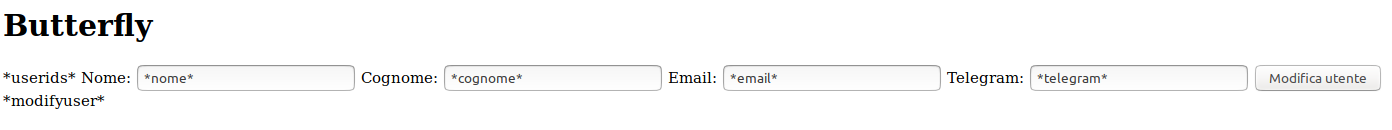
\includegraphics[width=\textwidth]{img/iscrizione_1.png}%TODO verificare immagine
	\caption{Interfaccia iscrizione nuovo utente}
\end{figure}
È anche possibile inserire un nuovo utente attraverso l'utilizzo delle \hyperref[APIRest]{API Rest}, come descritto nella sezione apposita.
Dopo aver effettuato l'iscrizione si è automaticamente autenticati all'interno del sistema. %TODO verificare

\subsubsection{Autenticazione}
È possibile effettuare l'autenticazione all'interno del sistema tramite il link del container sul quale è in esecuzione e specificato nella configurazione effettuata precedentemente.
Per effettuare correttamente l'autenticazione è necessario l'inserimento del proprio ID Telegram o Email con il quale si è iscritti nel sistema.
%TODO inserire immagine
In caso l'identificativo inserito non fosse valido, e non corrispondesse quindi ad un match nel database, verrà mostrato all'utente un messaggio di errore.
%TODO inserire immagine
Nel caso in cui un utente non autenticato cerchi di accedere ad una sezione per cui non ha i privilegi, questo verrà rimandato alla pagina di autenticazione.
%TODO verificare

\subsubsection{Pannello di controllo}
%TODO è veramente così?
Dopo aver effettuato l'accesso al sistema, si viene rimandati alla pagina relativa al Pannello di controllo che contiene i comandi principali per la navigazione del sito e che operazioni quindi un utente può eseguire.
Le pagine a cui si può navigare dal Pannello di controllo sono:
%TODO completare
\begin{itemize}
	\item pagina
\end{itemize}
\begin{figure}[H]
	\centering
	
\includegraphics[width=14cm]{img/pannello_1.png} %TODO verificare immagine
	\caption{Interfaccia modifica preferenze}
\end{figure}

\subsubsection{Modifica preferenze}
%TODO inserire immagine unica se si riescono a vedere tutte le impostazioni che possono essere modificate
La modifica delle preferenze è possibile solamente per utenti già iscritti ed autenticati nel sistema.
È raggiungibile tramite il Pannello di Controllo sotto la voce ... % TODO che voce
In questa sezione si possono trovare le principali impostazioni del sistema dal punto di vista dell'utente finale:
\begin{itemize}
	%TODO modificare in modo da non scrivere la parola utente?
	\item Come il sistema effettua la comunicazione con l'utente: modificare il proprio ID Telegram o indirizzo Email e impostare quale tra i due scegliere. Una modifica a questi campi comporta il cambiamento dell'identificativo utilizzato per accedere al sistema
	%TODO in caso ci fossero sia id telegram che indirizzo email che cosa si usa per l'autenticazione?
	\item Lista dei progetti disponibili e a cui si è iscritti. Un utente può essere iscritto a più progetti
	\item Modifica della priorità assegnata ad un progetto
	\item Lista dei Topic disponibili e iscrizione o disiscrizione da questi. Vengono mostrati in base ai progetti a cui si è iscritti.
	%TODO rivedere
	\item Lista delle keyword di interesse alle quali si è interessati, queste sono inserite in base al contenuto dei \texttt{commit\_message} che l'utente vuole ricevere
\end{itemize}
\begin{figure}[H]
	\centering
	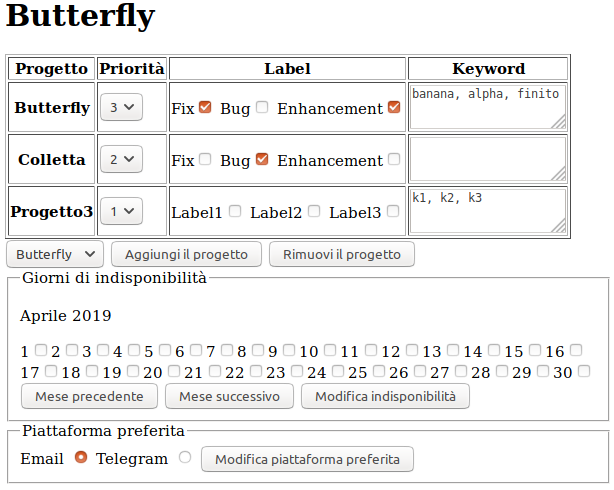
\includegraphics[width=\textwidth]{img/preferenze_1.png} %TODO verificare immagine
	\caption{Interfaccia modifica preferenze}
\end{figure}

\subsubsection{Inserimento giorni di indisponibilità}\label{indisponibilita}
Sempre dal Pannello di controllo è possibile raggiungere la pagina relativa alla disponibilità di calendario. 
%TODO verificare con Matteo
In questa è possibile specificare attraverso un calendario i giorni in cui non si è disponibili e quindi in caso di una notifica in arrivo mandarla ad un'altra persona che è in grado di gestirla.
%TODO inserire immagine di calendario
\begin{figure}[H]
	\centering
	%\includegraphics[width=\textwidth]{img/disponibilita_1.png} 
	\caption{Interfaccia iscrizione nuovo utente}
\end{figure}

\subsubsection{Uscita dal sistema}
%TODO spiegare
Per effettuare il logout dal sistema, cliccare su logout
%TODO inserire immagine

\subsubsection{Disiscrizione dal sistema}
%TODO verificare tutto
Viene data la possibilità di disiscriversi dal sistema ed eliminare quindi i propri dati all'interno di questo.
Per disiscriversi andare su ... dal pannello di controllo ...
\begin{figure}[H]
	\centering
	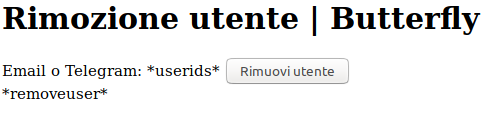
\includegraphics[width=10cm]{img/rimozione_1.png} %TODO verificare immagine
	\caption{Interfaccia iscrizione nuovo utente}
\end{figure}
Viene inoltre data la possibilità di disiscrivere un altro utente dal sistema facendo ...


%TODO da mettere un esempio per ciascuna
\subsection{API Rest}\label{APIRest}
\newcommand{\homeUrl}{home\_url}

Per la gestione delle risorse di \progetto\ abbiamo utilizzato lo standard architetturale delle API Rest.
Nelle sezioni successive viene descritto come interagire con le API fornite dal sistema.
Il root path sottinteso sarà sempre \texttt{\homeUrl/api/v1/}.
Ad esempio, per effettuare la GET degli user, l'indirizzo sarà:
\begin{center}
    \texttt{GET \homeUrl/api/v1/users}
\end{center}

\subsubsection{Users}

\texttt{Users} è la risorsa che corrisponde agli utenti.
È possibile visualizzare, aggiungere, modificare o rimuovere gli utenti tramite una semplice
richiesta HTTP.

\paragraph{Visualizzazione}

\begin{itemize}
    \item \textbf{Payload di tutti gli utenti}: \texttt{GET /users}
    \item \textbf{Utente specifico}: \texttt{GET /users/<id>}
\end{itemize}

\paragraph{Inserimento}
È possibile inserire un nuovo utente tramite la richiesta
    \begin{center}
        \texttt{POST /users}
    \end{center}

È possibile dare i seguenti campi di tipo stringa alla richiesta, per aggiungere in fase di creazione i dati:
\begin{itemize}[noitemsep]
    \item \texttt{name}
    \item \texttt{surname}
    \item \texttt{telegram}
    \item \texttt{email}
\end{itemize}
Almeno uno tra i campi \texttt{email} e \texttt{telegram} vanno fornite insieme al payload.

\paragraph{Modifica}

È possibile modificare un utente tramite la richiesta
\begin{center}
    \texttt{PUT /users/<id>}
\end{center}
È possibile dare i seguenti campi di tipo stringa alla richiesta, per aggiungere in fase di creazione i dati:
\begin{itemize}[noitemsep]
    \item \texttt{name}
    \item \texttt{surname}
    \item \texttt{telegram}
    \item \texttt{email}
\end{itemize}


\paragraph{Rimozione}

È possibile rimuovere un utente dal sistema \progetto\ con la richiesta
\begin{center}
    \texttt{DELETE /users/<id>}
\end{center}

Se il campo \texttt{<id>} corrisponde a un ID presente nel sistema, esso verrà rimosso.


\paragraph{Riepilogo}

\begin{table}[H]
    \begin{paddedtablex}[1.3]{\textwidth}{cYY}
        \thead{Metodo HTTP} & \thead{URI} & \thead{Action}\\\toprule
        \texttt{GET} & \texttt{/users} & Restituisce un payload in JSON di tutti gli utenti\\
        \texttt{GET} & \texttt{/users/<id>} & Restituisce un payload in JSON dell'utente che corrisponde a \texttt{<id>}\\
        \texttt{POST} & \texttt{/users} & Inserisce un nuovo utente. È necessario fornire uno tra i campi telegram o email\\
        \texttt{PUT} & \texttt{/users/<id>} & Modifica l'utente corrispondente a \texttt{<id>} con i campi passati nella richiesta\\
        \texttt{DELETE} & \texttt{/users/<id>} & Elimina l'utente corrispondente a \texttt{<id>} dal sistema\\
        \bottomrule
    \end{paddedtablex}
    \caption{Riepilogo delle Rest API per gli Users}
\end{table}


\subsubsection{Projects}

\paragraph{Visualizzazione}


\begin{itemize}
    \item \textbf{Payload di tutti i progetti}: \texttt{GET /projects}
    \item \textbf{Progetto specifico}: \texttt{GET /projects/<id>}
\end{itemize}

\paragraph{Inserimento}
È possibile inserire un nuovo progetto tramite la richiesta
    \begin{center}
        \texttt{POST /projects}
    \end{center}

È possibile dare i seguenti campi di tipo stringa alla richiesta, per aggiungere in fase di creazione
i dati:
\begin{itemize}[noitemsep]
    \item \texttt{url}
\end{itemize}


\paragraph{Modifica}

È possibile modificare un progetto tramite la richiesta
\begin{center}
    \texttt{PUT /projects/<id>}
\end{center}
È possibile dare i seguenti campi di tipo stringa alla richiesta, per aggiungere in fase di creazione
i dati:
\begin{itemize}[noitemsep]
    \item \texttt{url}
\end{itemize}


\paragraph{Rimozione}

È possibile rimuovere un progetto dal sistema Butterfly con la richiesta
\begin{center}
    \texttt{DELETE /projects/<id>}
\end{center}

Se il campo \texttt{<id>} corrisponde a un ID presente nel sistema, esso verrà rimosso.


\paragraph{Riepilogo}

\begin{table}[H]
    \begin{paddedtablex}[1.3]{\textwidth}{cYY}
        \thead{Metodo HTTP} & \thead{URI} & \thead{Action}\\\toprule
        \texttt{GET} & \texttt{/projects} & Restituisce un payload in JSON di tutti i progetti\\
        \texttt{GET} & \texttt{/projects/<id>} & Restituisce un payload in JSON del progetto che corrisponde a \texttt{<id>}\\
        \texttt{POST} & \texttt{/projects} & Inserisce un nuovo progetto\\
        \texttt{PUT} & \texttt{/projects/<id>} & Modifica il progetto corrispondente a \texttt{<id>} con i campi passati nel payload\\
        \texttt{DELETE} & \texttt{/projects/<id>} & Elimina il progetto corrispondente a \texttt{<id>} dal sistema\\
        \bottomrule
    \end{paddedtablex}
    \caption{Riepilogo delle Rest API per i progetti}
\end{table}

\subsection{Piattaforma di messaggistica}

\subsubsection{Email}

Per ricevere i messaggi di Butterfly tramite Email, è sufficiente fornire tramite l'interfaccia del Gestore Personale l'Email sulla quale si vuole ricevere la notifica.

\subsubsection{Telegram}

Per ricevere le notifiche via Telegram, è necessario fare un passaggio addizionale: va fornita l'autorizzazione al bot per poter inviare messaggi agli utenti. 
Il bot è raggiungibile al seguente link:
\begin{center}
    \url{http://t.me/ButterflyBot}
\end{center}

Dare il comando \texttt{/start} per dare l'autorizzazione di inoltro dei messaggi al bot.
È necessario inoltre aggiungere tramite l'interfaccia del Gestore Personale il proprio account Telegram.
In qualsiasi momento sarà possibile bloccare il bot in caso non si voglia più ricevere messaggi relativi a Butterfly su Telegram, tramite le funzionalità dell'applicazione.
Nel caso in cui si volesse utilizzare un altro bot, i passaggi da seguire possono essere trovati sulla pagina apposita della documentazione di Telegram\footnote{\url{https://core.telegram.org/bots}}.
%TODO aggiungere nome variabile
Per comunicare con questo bisogna modificare la variabile di ambiente ... che rappresenta il \texttt{token} univoco del nuovo bot, come descritto in \S\ref{var_consumer}.